\documentclass[modern]{aastex61}

\newcommand{\escapecmd}[1]{\texttt{\detokenize{#1}}}

\submitjournal{ApJ}

\shorttitle{Astropy Project II}
\shortauthors{Astropy Project et al.}

\begin{document}

\draft{\today}

\title{The Astropy Project: }

\correspondingauthor{Astropy Coordination Committee}
\email{coordinators@astropy.org}

\author{Astropy Collaboration}

\begin{abstract}
The Astropy project supports and fosters the development of open-source Python
packages that provide commonly-needed functionality to the astronomical
community.
A key element of the project is the Astropy core package, which serves as the
foundation for more specialized projects and packages.
In this article, we provide an overview of the organization of the Astropy
project and summarize key features in the core package as of the recent major
release, version 2.0.
We then describe the project infrastructure designed to facilitate [...]
We conclude with a future outlook of planned new features and directions for the
broader Astropy ecosystem.
\end{abstract}

%% Keywords should appear after the \end{abstract} command.
%% See the online documentation for the full list of available subject
%% keywords and the rules for their use.
\keywords{}

\section*{\textit{Notes and guidelines (to be removed)}}

\begin{itemize}
   \item The goal is to produce a brief and informative paper that covers major astropy principles not mentioned in the first paper, the core v2.0 package, and infrastructure in astropy project to support development in python.
	\item We don't plan on including code in this paper, but if you think you will need to include code in your section, please add it to a separate Python module (.py file) and include it in this repository.
    \item Use \escapecmd{\sectionname} not ``Section,'' \escapecmd{\figurename} not ``Figure''
    % I have never seen the \sectionname command and google is not any cleverer
    % Also, compilation fails when I use that. What's it good for?
    \item If your subpackage was included in Paper I, then please just include a note on what the package does, a reference to paper I, and any new major updates to your package
    \item If your subpackage was not included, then please a further description of the sub-package on level with what was in the first paper, and highlight any major features in it.   Typically length should be equivalent to one column
    \item Please make sure you are logged into Overleaf or pushing a commit with your information to be able to track the contributors to the paper.

\end{itemize}

\section{Introduction} \label{sec:intro}
% first draft by Moritz (hamogu)
All astronomical research makes use of software in some way and
astronomy as a field has long supported the development of specialized
software tools for different astronomical tasks. Some of those
software packages are (or at least were) supported by large
institutions, e.g.\ IRAF \citep[developed at NOAO,][]{IRAF}, MIDAS
\citep[developed at ESO,][]{MIDAS}, or ds9 \citep[developed at
% * <bsipocz@gmail.com> 2017-09-28T21:05:00.569Z:
% 
% > or ds9 
% probably starlink is a better example as being a large package of software similarly to IRAF and MIDAS rather than a single tool.
% 
% ^.
  SAO,][]{ds9}. These packages tend to address a wide range of users
and they typically provide some level of documentation and user
support. Other packages are developed foremost by individual research
groups and used mostly in work by members of this group. Those
packages can address more specialized needs, but are not necessarily
available to the community and even if they are, documentation can in
some cases be insufficient for new users and the quality of the
software, i.e. the robustness and the level of testing that has been
performed to ensure correctness, is not always clear. On the other
hand, there are also many widely used, well documented, high quality
software packages which are developed by individuals or small groups.

The implementation of astronomical software, be it for a package meant
for wide distribution or scripts and programs for a specific research
project, can be eased by the use of a library that provides core
functionality that is common to many astronomical tasks. Reading and
writing fits files is one example where it is time
consuming to implement the fits standard correctly and
programming is much faster when using an existing library perform this
task. Another example of such a common task is dealing with different
astronomical coordinate systems. The astropy project aims to provide a
library of core astronomical functionality in the Python programming
language.

Python\footnote{\url{https://www.python.org/}} is an increasingly
popular general-purpose scripting language that is available under a
permissive open source software licence free of charge for all major
operating systems. Stable and well-developed packages provide support
for array arithmetic \citep[numpy,][]{numpy}, a wide variety of
functions for scientific computing \citep[scipy,][]{numpy}, and
publication-quality plotting \citep[matplotlib,][]{matplotlib}. Tens of
thousands of other packages are available which can help with tasks
that are not astronomy specific but might be performed in the course
of astronomical research, e.g.\ presenting results on websites or
interfacing with databases.

At the same time, an ecosystem of tools, programs, and webservices
has become available that makes it easier to collaborate on code development,
continuously test the code, build and provide documentation, and
supply downloadable packages. The astropy project aims to develop and
provide high quality code and documentation according to the best
practices in software development. The project makes use of these
tools to do so without central institutional oversight.

The first public release of the astropy package is described in
\cite{2013A&A...558A..33A}. Since then, the astropy package has been
used in hundreds of projects, and the scope of the package as grown
considerably. At the same time, the community of astronomers
contributing to the project has grown tremendously and an ecosystem
of packages supporting or affiliated with the astropy core has
developed. In this paper, we describe the current status of the
astropy community, the astropy core package, and the astropy
ecosystem.

We start by describing the way the astropy project works and is
organized in section~\ref{sec:concepts}.  The project develops a core
package called \texttt{astropy} (section~\ref{sec:core}) and several
separate packages that help setting up the infrastructure for testing,
documentation etc.\ (section~\ref{sec:infrastructure}). In
section~\ref{sec:learning} we give an overview of the wealth of
resources created to teach new users the use of the astropy packages
and how to contribute to the community. We end with a short vision for
the future of astropy in section~\ref{sec:future}.



\section{Major concepts}
\label{sec:concepts}
% Anyone want to take this??
\subsection{APEs - Astropy Proposals for Enhancement}
% would be nice to write about the concept of APEs so we can refer to the
% relevant ones latr in the text

\subsection{Coordination of Astropy}
% Kelle

\subsection{Astropy development model, astropy ecosystem}
% Erik
This subsection should include some basic statistics about the contributors, commits, line of code etc. up to the 2.0 release when we know it.

\subsection{Concept of affiliated packages}
% it may be described in previous subsection, if not the Brigitta can try to
% write it up

\subsection{Mixin}

\subsection{Accuracy testing across many different implementation}

\subsection{Use of Quantities across package}
% Marten and Tom R.

{\bf Very rough first text!}

Historically, it has been unusual to keep units as part of numbers, especially as speed was often deemed essential and quantities used to be slower than regular arrays. Hence, programs and functions expected to be fed parameters in particular units, as (hopefully) stated in their documentation.  In astropy 0.4, therefore, unit and quantity support was still somewhat spotty, but this has changed greatly.  One of the riskiest classes was ngles, where both degrees and radians were ``obvious'' default units to some. As a consequence, quantities are most fully integrated in the coordinates module (Sect.~\ref{sec:coordinates}). In astropy 2.0, one can also opt in to use quantities fully in tables, by using the {\tt QTable} class (see Sect.~\ref{sec:table}). As a result, units in fits tables are also well-supported. For most other modules, quantities are at least accepted, and often assumed by default.

In the process, some standard wrappers have been defined that make defining functions that require quantities as input simpler. As an extension of this, we plan to define wrappers for functions that work on numbers that will automatically convert quantities to any required units.

\subsection{Release cycle and Long Term Support}
% This could also include information about the development cycle
% Brigitta can writes this up if there's no other taker
%
% - reference APE2 for versioning and APE10 for dropping python2 support
% - shall we maybe refer to the release calendar, too?
% - should we mention that v3.0 is the exception to the version numbering
%   scheme we use by not being 2.1?
\par The general scheme for the releases and version numbering that the core
package has adopted if the following. Astropy has new feature releases every
6 month, and between feature releases additional bugfix releases that
contain only bugfixes but no new features. The timing of
%
\par Long-term support (LTS) releases continue to receive bugfixes for 2
years with no changes to the API. They are ideal for pipelines and other
applications where API stability is essential. The latest LTS release is
also the last one that supports Python2, and will receive bug fixes until the
end of 2019.
%
\par The version numbering of astropy reflects on the release scheme
described above. The core package uses the form x.y.z, where x is advances
on LTS, y is advanced for a non-LTS feature release, and z is advanced on
bugfix releases.

%\subsection{Difficulty of reversing design choices}
%Deciding if a feature should be included
%difficulty to decide where general use ends and "handy feature for some" starts, i.e. how to reject PRs or deal with maintenance burden

\section{Astropy Core Package v2.0}
\label{sec:core}
The astropy project aims to provide python-based packages for all tasks that are commonly needed in a large subset of the astronomical community. Two aspects of this (time and coordinate transformations) are already discussed in great detail in section 3. In this section, we highlight other features introduced or substantially improved since version v0.2, which is described in \citet{2013A&A...558A..33A}.
(ordered in the order in which they appear in the astropy documentation)

% \subsection{Analytic Functions}
% moved to models and depreciated --
% just here for completeness at the moment

\subsection{Units and quantities}
\label{sec:units}
% Marten, Adrian

\textbf{Key features:}
\begin{itemize}
	\item incl logarithmic units and magnitudes
	\item speed improvements
    \item interaction with numpy arrays
\end{itemize}

\subsection{Constants}
% David S.
versioning


\subsection{Coordinates}
\label{sec:coordinates}
% Adrian, Erik

The \texttt{astropy.coordinates} subpackage is designed to support representing
and transforming celestial coordinates and, new in version 2.0, velocities.


- Three-tiered structure for coordinates: representation, frame, skycoord
- With differential classes, frames support velocities

Accuracy and comparison of coordinate system definitions?

\textbf{Key features:}
\begin{itemize}
	\item Celestial coordinates, and local coordinates (via EarthLocation + Time)
	\item JPL ephemerids
    \item Proper motions, radial velocities
\end{itemize}

Separately, talk about representations as vectors? (MHvK)

\subsection{Time}
\label{sec:time}

Q: does it make sense to refer forward to fits support, even though it is 3.0?

\subsection{Data arrays}

\subsubsection{NDDdata}
% Matt C., Michael, or Steve C.
% Larry (nddata.utils)
%NOTE (Larry), The package is nddata, which includes the NDData object.  %Don't forget the nddata.utils functionality (e.g. Cutout2D, block\_reduce, %etc.).

\subsubsection{Tables}
\label{sec:table}
% Tom A.
QTable is new, mixin columns for time and coordinates. Table operations were added in v0.3

\subsection{io}
% Simon

\subsubsection{Unified file read/write interface}

Check when it was added (0.3?). Overview of the supported formats (ascii, fits, votable).

\subsubsection{Enhanced CSV format}

\subsubsection{ASCII, FITS, etc.}

One subsection per format (if enough new features) ?

\begin{itemize}
\item ascii : fast reader/writer (1.0), HTML tables
\item fits: lazy loading, command-line scripts (fitsheader, fitsinfo)
\end{itemize}

\subsection{Modeling}
\label{sec:modeling}
% Nadia
% Lim blackbody
% Tom R. -- unit support
The whole modeling submodule was missing from the previous paper, so everything really, including compound models, unit support etc.

\subsection{Convolution}
% Adam G.

astropy implements `normalized convolution' \citep[e.g.,][]{Knutsson1993}, which is an image reconstruction technique in which missing data are ignored during the convolution and replaced with values interpolated using the kernel.   In version $<=1.3$, the direct convolution and fft convolution approaches were not consistent, with fft convolution implementing normalized convolution and direct convolution implementing a different approach.  As of v2.0, the two methods are consistent and include a suite of consistency checks.


\begin{figure}
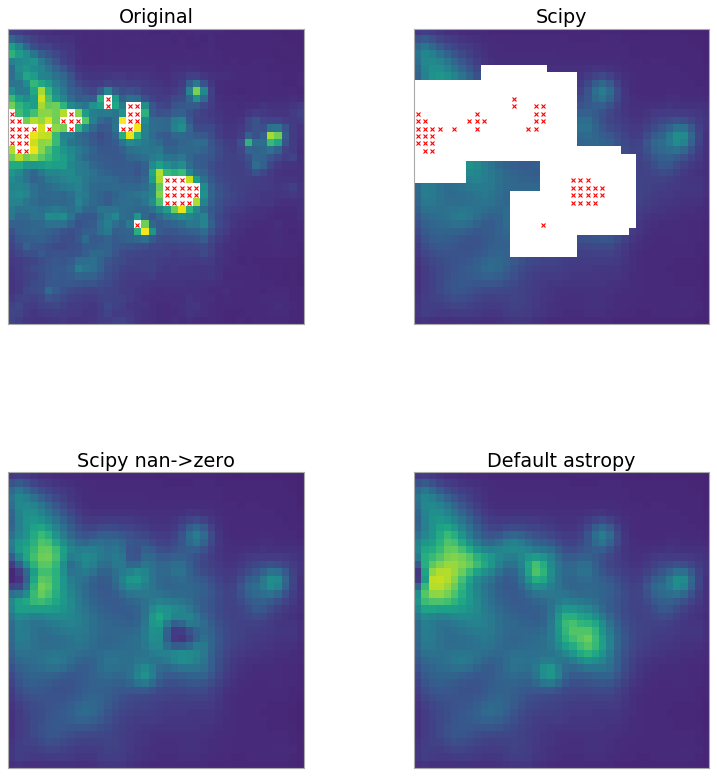
\includegraphics[width=\textwidth]{convolution_example.png}
An example showing different modes of convolution available in the python ecosystem.  The red x's mark pixels that are set to NaN in the original data (a).  If the data are convolved with a Gaussian kernel on a 9x9 grid using scipy's direct convolution (b), any pixel within range of the original NaN pixels is also set to NaN.  Panel (c) shows what happens if the NaNs are set to zero first: the originally NaN regions are depressed relative to their surroundings.  Finally, panel (d) shows astropy's convolution behavior, where the missing pixels are replaced with values interpolated from their surroundings using the convolution kernel.
\end{figure}


\subsection{Visualization}
% Larry:  Image visualization (stretching, scaling), RGB
% Tom R.:  WCSAxes

wcsaxis, rgb, histograms comes to mind.Can use more publicity and also makes good images to include in the paper.


%\subsection{Utils}
% Lim

\subsection{Cosmology}


\subsection{Statistics}
% Steve C.: overview, circular stats, 
% Jake V.:  Lomb-scargle, Bayesian blocks
% Larry:  sigma clipping, biweight stats
% Ze':  Ripley's K (spatial stats)
major additions to be discussed: lomb-scargle, sigma clipping, bayesian blocks, histograms, also:  robust (biweight) statistics

\subsection{Robust Statistical Estimators}
\subsection{Circular Statistics}
\subsection{Lomb-Scargle Periodograms}
\subsection{Ripley's K Function Estimators}
\subsection{Histogram Binning}

\section{Infrastructure for affiliated packages}
\label{sec:infrastructure}
% - should we use links to the appropriate github repo?
%
\par In addition to astronomy related packages and libraries, the Astropy
Project also contains and supports several infrastructure package that are
very generic. The following sections describes the most widely used
selection of them.
%
\subsubsection{Package template}
% Brigitta may write this up if there is no other takers
\par Astropy provides a template package that any Python package is welcome to
use (many affiliated packages do so). The template contains a ready-to-go
package layout. It provides infrastructure such as documentation tools,
testing framework and CI templates and configurations, Cython integration,
and documentation on how to make it all work.
%
\subsection{Continuous integration helpers}
% Brigitta
\texttt{ci-helpers} is a collection of scripts that empowers package
maintainers to control their testing set up and installation process for
various continuous integration services via a set of environment
variables. While the current development is mostly driven by the needs of
the astropy ecosystem, the actual usage of this package is extremely
widespread. Currently we support setups for TravisCI and AppveyorCI.
%
\subsection{sphinx extensions}
% Tom R


% \section{State of the Ecosystem}
% Commenting out unless a clear statement is added

\section{Learning Astropy}
\label{sec:learning}
% Kelle, Adrian
% - would astropy learn mature enough to described in the paper, or maybe it should go as a subsection for the next, future of astropy section?

Explain components: Documentation, Example gallery, Tutorials and lessons

\section{The future of the Astropy project}
\label{sec:future}

dropping python2 support, growths of affiliated packages
Summary

\acknowledgments

Who to thank?  numfocus,

%% Similar to \facility{}, there is the optional \software command to allow
%% authors a place to specify which programs were used during the creation of
%% the manusscript. Authors should list each code and include either a
%% citation or url to the code inside ()s when available.

\software{astropy \citep{2013A&A...558A..33A},
          numpy,
          scipy,
          }

\bibliographystyle{aasjournal}
\bibliography{bibliography}

\begin{thebibliography}{}

\end{thebibliography}



\end{document}

